\section{Description and Methodology}\label{chapter:Description and Methodology}
This section covers how the assignment was solved and different design choices. This was done in the following steps:

\begin{itemize}
	\item Configure and build uClinux and flash it to the board.  
	\item Create a device driver for the gamepad.
	\item Create a device driver to provide timer support. 
	\item Create the game. 
	\item Attempt to make a sound device driver. 
\end{itemize}


\subsection{Installing uClinux}
 

We were provided with a skeleton code which contained the source code for uClinux and skeleton code for the driver and the game. The build tool ptxdist was used to compile the kernel, the modules and other software, package it into a binary file and flashing it to the development board. The compendium gave very clear directions on how this should be done\cite{compendium}.

After configuring the ptxdist project, the project was build and flash by the following commands:
\hfill \\
\hfill \\
\texttt{ptxdist images} 
\hfill \\
\hfill \\
\texttt{ptxdist test flash-all}
\hfill \\
\hfill \\
But when we were working on the drivers, it would be too time consuming to rebuild and flash the whole project. Thus the compendium provided an alternative route for only building and flashing the respective modules. There were some problems with the provided route though, because the modules would not update. We solved it by doing the following commands when flashing the drivers/applications:

\begin{enumerate}
	\item \texttt{ptxdist clean <packagename>}
	\item \texttt{ptxdist go}
	\item \texttt{ptxdist image root.romfs}
	\item \texttt{ptxdist flash-rootfs} 
\end{enumerate}

We were able to interact with the Linux OS on the development card by using a provided program called \textit{miniterm}, which allowed us to interact with it as a standard shell. 

\subsection{The Gamepad Driver}

This driver should allow the userspace to read the status of the gamepad buttons. We also added interrupt support, and userspace signaling support, but later decided that this was better left to the timer driver. Thus, details on how interrupt and signaling support was implemented will be covered in the next section. 

From the start of the development we wanted to make this driver as dynamic as possible, i.e. dynamically allocate all needed resources, making it more portable. The compendium provided most of the steps required for allocating the neccessary resources, making the driver interface available for the OS and visible in userspace:

\begin{itemize}
 \item Allocate a device number for the device using \texttt{alloc\_chrdev\_region(...)}.
 \item Provide functions to the operating systems, so the device can be accessed by user applications as a file, using a \texttt{file\_operations} struct and the function \texttt{cdev\_init(...)}. 
 \item Add the driver to the system using \texttt{cdev\_add(...)}.
 \item Make the driver visible in user space using \texttt{class} struct, initalize it with \texttt{class\_create(...)}, and then create the device and register it with sysfs using the fuction \texttt{device\_create(...)}
\end{itemize}

In order to make sure that no other process was using the hardware, all the hardware's memory region was allocated using \texttt{request\_mem\_region(...)} when the driver was initalized. When the driver is removed, all the resources was released with \texttt{release\_mem\_region(...)}. For this driver we had to allocate the \textit{GPIO\_PC} region for reading button status, \textit{GPIO\_PA} region for output (used during testing) and some registers for interrupts. 

Even though we are not using virtual memory in this assignment, we decided to program our drivers as if they were. This makes the driver more robust, as it follows the Linux standard and can thus potentially harvest all the benefits of virtual memory. We thus had to use \texttt{ioremap\_nocache(...)} function to memory map the memory regions, and read/write to them using \texttt{ioread32(...)} and \texttt{iowrite32(...)}, respectively.

In order for the userspace to read the button status, the driver provides a \texttt{read(...)} function. The function contains the parameter \texttt{char \_\_user *buff}, which is a pointer to a buffer that the calling user application can access. Thus the driver writes the first eight bits of the register \textit{GPIO\_PC\_DIN} (which represents the button status) to that buffer.

\subsection{The Timer Driver}

The main reason for the timer driver was to provide an easy way to calculate when the game should update the frame. This was initially needed to make the astroids move downwards on specfic itervals. Using the code provided by \cite{timerguide} we were provided an interrupt timer that we could specify in miliseconds. Since the frame had to be updated several times a second, we decided that we thus did not need the gamepad driver to let the game know a button had been pushed. Instead we read the button status every time the timer signaled the game, for two reasons: 

\begin{itemize}
	\item Easier programming. Do not have to decide which driver that sent the signal to the game.
	\item Smoother gameplay. Since the gamepad is read several times a second, you can move the shield by simply keep pressing a button. Instead of having to stutter moving by creating an interrupt. And since the interrupts from the timer is needed for moving the astroid, checking the gamepad, while we are at it, does not hurt the energy efficiency. 
\end{itemize}

The interaction between the game, gamepad driver and timer driver and be seen in figure \ref{game_drivers}.

\hfill \\

\begin{figure}[ht]
    \centering
      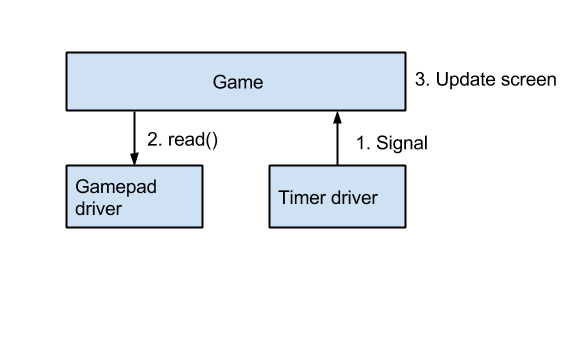
\includegraphics[width=9cm]{figures/Drivers_gamepad_interact}
    \caption{The interaction between the drivers and the game.}
    \label{game_drivers}
\end{figure}


The timer followed the same steppes as the gamepad driver for initalization, resource allocation, providing functions to userspace and making itself visbile to userspace. But in addition it had to provide signal support, in order to signal the game whenever the timer was finished. \textit{Linux Device Drivers}\cite{LDD} provided the neccessary information to enable device-user application-signaling.  

This was done by providing a \texttt{fasync(...)} function to userspace, which a user application could use to register itself as a listener to signals from the driver. All the listeners to the driver is stored in a \texttt{fasync\_struct} struct, and are added by calling the \texttt{fasync\_helper(...)} function. In order to signal the user application the function \texttt{kill\_fasync(...)} was called in the timer callback function (i.e. whenever the timer was finished). The user application was removed from the listener list by calling  \texttt{fasync\_helper(...)} upon close, with -1 as \textit{file\_descriptor}. 

But in order for the user application to add itself as a listener, it had to execute the following code: 

\begin{lstlisting}[frame=single]  % Start your code-block

signal(SIGIO, &signal_handler);
fcntl(fd, F_SETOWN, getpid());
oflags_dg = fcntl(fd_dg, F_GETFL);
fcntl(fd, F_SETFL, oflags_dg | FASYNC);

\end{lstlisting}

Where \textit{fd} is the file descriptor and \textit{signal\_handler} is the function that will be called when a signal from the driver occurs. 

\hfill \\

The timer driver also provided a \texttt{write(...)} function, where the user could specify the number of miliseconds the timer should run for, before signaling the user application. It also provides a \texttt{read(...)} function, that returns 1 if the timer is running.  

\subsection{The Game} 

The game itself is very simple. It uses the \textit{framebuffer}, located at \texttt{/dev/fb0}, to render the screen. For easier development and code the framebuffer was memory mapped, which allowed us treat it as a reqular C array. It also allowed to decide which part of the screen should be rerendered, using the \texttt{fb\_copyarea} struct and the framebuffer's \texttt{ioct1(...)} function. Thereby saving enegy, since we do not have to rerender the whole screen when only a small part needs to be updated.

As mentioned before the game uses the gamepad driver to read the status of the gamepad buttons, and the timer driver to recognize when it needs to update the screen (see figure \ref{figure_game}). Low update intervals gives good performance, but comes with a energy cost. The more you update the screen, the smoother it is, but uses a lot more energy. This will be discussed in more detail in the result section. 

The game is interrupt-driven, and sleeps whenever it does not have to handle a signal from the timer driver. Thus it uses as little energy as possible.

As the game implementation was really simple, and a rather uimportant part of the excerise, we will not go into any more detail on the implementation. Interested readers can read the provided code. 

\subsection{The Sound Driver}

We wanted to have sound to our game, so we tried to implement a sound driver. On our first attempt we tried by doing it the same way as in the previous assignment, where we made the CPU write directly to the \textit{Digital to Analog Converter} (DAC). It worked, but the sound quality was \emph{really} bad, due to performance issues. Thus we tried implementing it using \textit{Direct Memory Access} (DMA), but it did not work. This section will cover our attempted solution.  

We initalized the driver in the same way as the previous drivers, so what remained was setting up the interaction between the DMA, DAC, TIMER3 and the driver. The interaction is illustrated in figure \ref{figure_dma}.

\begin{figure}[ht]
    \centering
      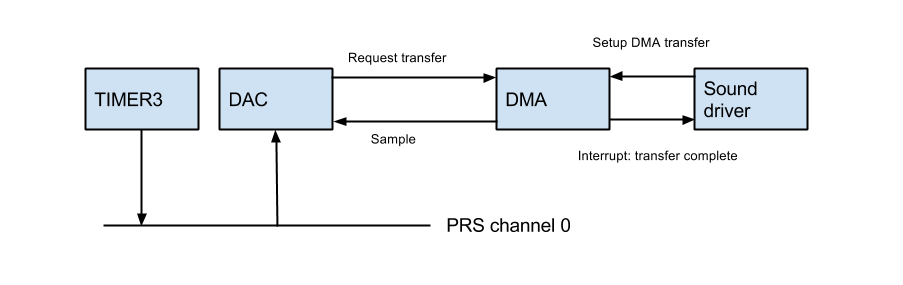
\includegraphics[width=9cm]{figures/DMA}
    \caption{The interactions between the DAC, DMA, TIMER3 and CPU.}
    \label{figure_dma}
\end{figure}

It works as follows:

\begin{itemize}
	\item TIMER3 underflow is set to PRS channel 0 input.
	\item DAC channel 0 and 1 is set convert data on PRS channel 0 input.
	\item The DMA is set up for basic transfer. It triggers on DAC conversion complete, and arbitrate after after each transfer. Thus allowing the DAC to control the speed of the data transfer. When the DMA has transfered all of the provided samples, it sends an interrupt to the sound driver - which should provide it with more samples to transfer.
	\item The sound driver has access to an array of sound samples it should provide the DMA with. This is done by updating the DMA descriptor, which contains the source end address, destination end address and control bits. The control bits specifies the size of each transfer, how the source and destination addresses should be incremented, and the number of transfers (up to 1024) etc. Thus when the DMA has transfered 1024 samples, the sound driver has to provide it with the address of the next 1024 samples, until all the samples have been transfered.  
\end{itemize}

But for unknown reasons this did not work, and after hours of debugging we were forced to give up. 






